\documentclass{amsart}

\usepackage{amssymb}
\usepackage{amsmath}
\usepackage{alltt}
\usepackage[dvipsnames]{xcolor}
\usepackage{tkz-graph}

\title{Probability: Final Exam}
\author{Mark Ditsworth}

\begin{document}
	\maketitle
	\section{Problem 1}
	\subsection{Part I}
	Alice and Bob each choose a number independently and uniformly random from the interval $[0,2]$. Consider the following events:\\
	\textbf{A}. the absolute difference between the two numbers is greater than 1/4.\\
	\textbf{B}. Alice's number is greater than 1/4.\\
	Find $\mathbf{P}(A\cap B)$.\\
	\\
	This is the fraction of the area of a $2\times 2$ square that satisfies both conditions if the $x$ and $y$ axes are Alice's and Bob's numbers, respectively. The inclusive area is made up of two isosceles right triangels with side lengths of 1.75 and 1.5, respectively. The combined area is
	\[
	\frac{1}{2}(1.75)^2 + \frac{1}{2}(1.5)^2 = 2.65625
	\]
	Thus, $\mathbf{P}(A\cap B) = \frac{2.65625}{4} = \frac{85}{128}$.
	\\
	\subsection{Part II}
	There are $m$ red balls and $n$ white balls in an urn. We draw two balls at random without replacement. What is the probability that the balls are a different color?\\
	\\
	This is the sum of two probabilities: drawing a red then white, and drawing a white then red.
	\[
	\frac{m}{m+n}\frac{n}{m+n-1} + \frac{n}{m+n}\frac{n}{m+n-1} = \frac{2mn}{(m+n)(m+n-1)}
	\]
	\\
	\subsection{Part III}
	20 black pebbles are arranged in 4 rows of 5 pebbles each. We choose 4 at random and color them red. What is the probability that each red pebble lies in a different row?\\
	\\
	There are $5^4$ possible orderings of 4 pebbles in different rows (5 places for the first, 5 places for the second, etc.). There are $\binom{20}{4}$ total permutations of the pebble sequences. Thus, the probability is
	\[
	\frac{5^4}{\binom{20}{4}} = \frac{5^4 4!16!}{20!}
	\]
	\\
	\subsection{Part IV}
	We have two light bulbs, A and B. Bulb A has an exponentially distributed lifetime with mean of 4 days. Bulb B has an exponentially distributed lifetime with mean 6 days. We select one bulb at random (each is equally likely). Given that the bulb has been working for 12 hours, what is the probability that we chose bulb A?\\
	\\
	By Bayes theorem, we have
	\[
	P(\text{selecting A}|l.t.>\text{0.5 days})=
	\frac{P(\text{selecting A})P(l.t.>\text{0.5 days}|\text{selecting A})}{P(l.t.>\text{0.5 days})}
	\]
	For an exponential random variable, $P(l.t.> t)=
	e^{\frac{1}{\mu}t}$.
	Thus, we have
	\[
	\frac{(0.5)e^{\frac{1}{4}\frac{1}{2}}}{0.5(e^{\frac{1}{4}\frac{1}{2}}+e^{\frac{1}{6}\frac{1}{2}})} = \frac{1}{1+e^{1/12 - 1/8}} = \frac{1}{1+e^{1/24}}
	\]
	\\
	\subsection{Part V}
	A test for a rare disease is correct 95\% of the time. A false positive has a probability 0.95 and a false negative has a probability 0.95. A random person drawn fro the population has a probability of 0.001 of having the disease. Given that a person just tested positive, what is the probability of having the disease?\\
	\\
	By Bayes theorem,\\
	$P(\text{sick}|\text{positive})=
	\frac{P(\text{sick})P(\text{positive}|\text{sick})}{P(\text{positive})} = \frac{(0.001)(0.95)}{(0.001)(0.95)+(0.999)(0.05)}=0.187$
	\\
	\subsection{Part VI}
	Let $X$ be a random variable with
	\[
	f_X(x) = 
	\begin{cases}
		 2e^{-2x} & x\geq 0\\
		 0 & \text{otherwise}
	\end{cases}
	\]
	Let $Y=2X-4$. Find $f_Y(0)$.\\
	\\
	\[
	F_Y(y) = P(Y\leq y) = P\left(X \leq \frac{y}{2}+2\right) = F_X\left(\frac{y}{2}+2\right)
	\]
	\[
	\frac{d}{dy}F_Y(y) = \frac{d}{dy}F_X\left(\frac{y}{2}+2\right)
	\]
	\[
	f_Y(y) = \frac{1}{2}f_X\left(\frac{y}{2}+2\right)
	\]
	\[
	f_Y(0) = \frac{1}{2}f_X(2)= e^{-4}
	\]
	\\
	\subsection{Part VII}
	$X$ and $Y$ are independent random variables. $X$ is exponentially distributed with mean $1/3$. $Y$ is Bernoulli with $p=1/2$. Let $Z=X+Y$. What is the transform of $Z$, $M_Z(s)$ evaluated at $s=1$?\\
	\\
	\[
	M_X(s) = \frac{3}{3-s} \qquad, \qquad M_Y(s) = \frac{1}{2}+\frac{1}{2}e^s
	\]
	Since the PDF of $Z$ is the convolution of $X$ and $Y$, in the $s$ domain it is the multiplication of $M_X(s)$ and $M_Y(s)$.
	\[
	M_Z(s) = M_X(s)~M_Y(s)
	\]
	\[
	M_Z(1) = \frac{3}{2}\left(\frac{1}{2}+\frac{1}{2}e\right)=
	\frac{3}{4}(1+e)
	\]
	\\
	\subsection{Part VIII}
	A number $p$ is chosen at random from a uniform distribution $[0,1]$. A sequence of $k$ Bernoulli trials is then performed each with a success probability of $p$. What is the variance of the number of successes in the $k$ trials?\\
	\\
	By the law of total variance,
	\[
	\text{Var}(X) = \textbf{E}[\text{Var}(X|P)] + \text{Var}(\mathbf{E}[X|P])
	\]
	\[
	= \textbf{E}[kP(1-P)] + \text{Var}(kP)
	\]
	\[
	=k\textbf{E}[P] - k\textbf{E}[P^2] + k^2\text{Var}(P)
	\]
	\[
	=k\textbf{E}[P] -k\textbf{E}[P^2] + k\textbf{E}[P]^2 - k\textbf{E}[P]^2 + k^2\text{Var}(P)
	\]
	\[
	=k\textbf{E}[P] - k\text{Var}(P) -k\textbf{E}[P]^2 + k^2\text{Var}(P)
	\]
	\[
	=\frac{k}{2} - \frac{k}{12} - \frac{k}{4} + \frac{k^2}{12} = \frac{k}{6}+\frac{k^2}{12}
	\]
	\[
	=\frac{k(2+k)}{12}
	\]
	\\
	\subsection{Part IX}
	A police radar always over-estimates the speed of a car by an amount that is uniformly distributed between 0 and 5 mph. Assume that car speeds are uniformly distributed between 60 and 75 mph and are independent of the radar over-estimate. If the radar measures a speed of 76 mph, what is the least-squares estimate of the actual car speed?\\
	\\
	The least squares estimate of $Y$ is \textbf{E}[$Y|X$]. Given the radar speed of 76 mph. The possible values of the actual speed are uniformly distributed between 71 and 75 (since 75 is the maximum speed). Thus, the least squares estimate is $\frac{75+71}{2} = 73$ mph.
	\\
	\subsection{Part X}
	A mosquito lands on your back and bites according to a Bernoulli process. The expected time of the first bite is 10 seconds. What is the probability that the second bite occurs at exactly 10 seconds?\\
	\\
	The time to first arrival is a geometric distribution, with the average time equal to $\frac{1}{p}$. Thus, $p=0.1$.
	
	The $k$th arrival time of a Bernoulli process is modeled by the Pascal distribution, where $P_k(t)
	= \binom{t-1}{k-1}p^k (1-p)^{t-k}$.
	\[
	P_2(10) = \binom{10-1}{2-1}\left(\frac{1}{10}\right)^2\left(\frac{9}{10}\right)^{10-2} = \frac{9!}{8!}\frac{9^8}{10^2 10^8} = \frac{9^9}{10^{10}} \approx 0.0387
	\]
	\subsection{Part XI}
	In order to estimate $p$, the fraction of people who will vote for candidate A in the next election, you conduct a poll of $n$ people drawn randomly and independently from the population Your estimator $M_n$ is obtained by dividing $S_n$, the number of people voting for candidate A in the sample, by $n$. Find the smallest value of $n$ needed to guarantee that
	\[
	\mathbf{P}(|M_n - p|\geq 0.01) \leq 0.01
	\]
	Applying the WLLN to the Chebyshev inequality, we have
	\[
	\mathbf{P}(|X-\mu|\geq \epsilon) \leq \frac{\sigma^2}{n\epsilon^2}
	\]
	Since each sampled person's vote is a Bernoulli distribution, we have $sigma^2 = p(1-p)$ and $p(1-p)\leq \frac{1}{4}$ for all $p\in [0,1]$. Thus,
	\[
	\mathbf{P}(|M_n-p|\geq 0.01) \leq \frac{\sigma^2}{n(0.01)^2}\leq \frac{1}{n(4)(0.01)^2} \leq 0.01
	\]
	\[
	n \geq \frac{1}{4(0.01)^3} = 250,000
	\]
	\subsection{Part XII}
	It rains each day with a probability 0.1, independent of all other days. Use the CLT to approximate the probability that out of 365 days in the year, it will rain on at least 100 days. How good is this approximation?\\
	\\
	The precipitation state on a given day $X_i$ is Bernoulli with $p=0.1$. Thus the average value for a day $\mu=0.1$, and the variance $\sigma^2=p(p-1)=0.09$.
	\\
	Let $S_n = X_1 + X_2 + \dots +X_n$.
	\[
	\mathbf{P}(S_{n=365}\leq 100) = \Phi\left(
	\frac{100 - 365\mu}{\sigma\sqrt{365}}
	\right)=\Phi\left(\frac{635}{3\sqrt{365}}
	\right)
	\]
	So, $\mathbf{P}(S_n\geq 100) = 1 - \Phi\left(\frac{635}{3\sqrt{(365)}}\right) \approx 0$\\
	\\
	The true distribution is Binomial with $p(k) = \binom{365}{k}p^k(1-p)^{365-k}$\\\\
	\[
	\mathbf{P}(k\geq 100) = 1 -\mathbf{P}(k \leq 99) = 1-\sum_{i=0}^{99}\binom{365}{i}p^i(1-p)^{365-i} = 1.11\times 10^{-16} \approx 0
	\]
	The difference between this answer and the approximation with the CLT is within computational rounding difference.
	\pagebreak
	\section{Problem 2}
	Deer come to a river according to a Poisson process with arrival rate $\lambda_d=8$ per hour; elephants come to the river by an independent Poisson process with arrival rate $\lambda_e=2$ per hour. Assume that elephants and deer are the only animals that go to the river.
	\\
	\subsection{Part A}
	Let $N$ be the number of animals you see during the first 3 hours. Find $\mathbf{E}[N]$ and Var$(N)$.\\
	\\
	Let $D$ and $E$ be the number of deer and elephants seen in the first 3 hours, respectively.
	\[
	p_D(k) = \frac{(3\lambda_d)^k e^{-3\lambda_d}}{k!}
	\rightarrow M_D(s) = e^{e\lambda_d(e^s-1)}
	\]
	\[
	p_E(k) = \frac{(3\lambda_e)^k e^{-3\lambda_e}}{k!}
	\rightarrow M_E(s) = e^{e\lambda_e(e^s-1)}
	\]
	\[
	N = D + E \rightarrow M_N(s) = M_D(s)~M_E(s) = 
	e^{3(\lambda_d+\lambda_e)(e^s-1)}
	\]
	$N$ is therefore a Poisson process with intensity $3(\lambda_d+\lambda_e) = 30$. So, 
	\[
	\mathbf{E}[N] = 30 \qquad , \qquad \text{Var}(N)=30
	\]
	\subsection{Part B}
	What is the probability of seeing your 3rd elephant before your 9th deer?\\
	\\
	The $k$th arrival time in a Poisson process follows an Erlang distribution,
	\[
	f_{Y_k}(y) = \frac{\lambda^k y^{k-1}e^{-\lambda y}}{(k-1)!}
	\]
	We can determine this probability through Monte Carlo simulations of the difference in time between the third elephant's arrival and the ninth deer's arrival. The fraction of (a large number of) simulations for which this difference is negative will approach the probability that the third elephant comes first.
	
	\begin{alltt}
	\textcolor{ForestGreen}{In [1]:} \textcolor{OliveGreen}{import} \textcolor{blue}{numpy} \textcolor{OliveGreen}{as} \textcolor{blue}{np}
	\textcolor{ForestGreen}{In [2]:} \textcolor{OliveGreen}{from} \textcolor{blue}{scipy.stats} \textcolor{OliveGreen}{import} erlang
	\textcolor{ForestGreen}{In [3]:} lambda_e = 2.
	\textcolor{ForestGreen}{In [4]:} lambda_d = 8.
	\textcolor{ForestGreen}{In [5]:} third_ele_times = erlang.rvs(3,scale=1/lambda_e,size=5000000)
	\textcolor{ForestGreen}{In [6]:} ninth_deer_times = erlang.rvs(9,scale=1/lambda_d,size=5000000)
	\textcolor{ForestGreen}{In [7]:} diff = third_ele_times - ninth_deer_times
	\textcolor{ForestGreen}{In [8]:} len(np.where(diff<0)[0])/5000000.
	\textcolor{red}{Out[8]:} 0.382903
	\end{alltt}

	Therefore, we about a 38\% probability of seeing our third elephant before our ninth deer.
	
	\subsection{Part C}
	At the end of 3 hours, you have seen 24 deer but no elephants. What is the probability that you will see an elephant in the next hour?\\
	\\
	Since the deer and elephant arrival processes are independent, we can ignore the 24 deer information. Further, since Poisson process is memoryless, the fact that no elephants have been seen in the first three nours has no bearing on the probability of occurrence in the future.
	
	The number of elephants seen in a one hour time block is a Poisson random variable with PMF $\frac{\lambda_e^k e^{-\lambda_e}}{k!}$. The probability of seeing \textit{no} elephants in the next hour is $e^{-\lambda_e} = e^{-2}$. Thus, the probability of seeing at least one elephant within the hour is $1-e^{-2}$.
	\\
	\subsection{Part D}
	It has been 6 hours since you have started watching. You have seen 53 deer and no elephants. How many more deer do you expect to see before you see your first elephant?\\
	\\
	Again, since Poisson processes are memoryless, the 6 hours and 53 deer are irrelevant information. At the present moment, the expected arrival time of the first elephant $\mathbf{E}[T] = \frac{1}{\lambda_e}=0.5$ hours. We set this time as $tau$. The expected number of deer seen in $\tau$ units of time is $\lambda_d \tau = 8(0.5)=4$
	\\
	\subsection{Part E}
	You plan on staying at the river until you have both a picture of a deer and an elephant. How long do you expect to stay?\\
	\\
	The arrival rate for a general animal is the sum of the arrival rates for elephants and deer, $\lambda_e + \lambda_d = 10$. Thus, the expected wait time for the first animal of any kind is $\frac{1}{10}$ hour.
	
	There are then two possibilities, a deer was the first to show up (with probability $\frac{\lambda_d}{\lambda_d+\lambda_e}$), and we wait for an elephant (average time of $\frac{1}{\lambda_e}$); or the first animal was an elephant (probability $\frac{\lambda_e}{\lambda_d+\lambda_e}$), and we wait for a deer (average time of $\frac{1}{\lambda_d}$)
	
	In total, our expected wait time is
	\[
	\frac{1}{\lambda_d+\lambda_e} + \frac{\lambda_d}{\lambda_d+\lambda_e}\frac{1}{\lambda_e}
	+\frac{\lambda_e}{\lambda_d + \lambda_e}\frac{1}{\lambda_d} = \frac{1}{10}+\frac{4}{(5)(2)}+\frac{1}{(5)(8)}=\frac{21}{40}
	\]
	\\
	\subsection{Part F}
	Each time you take a picture, there is a probability of 0.1 that the picture turns our poor. You take a picture each time an animal arrives to the river. let $X$ be the time (in hours) until you get your third picture of an elephant. Find the PDF of $X$.\\
	\\
	This is a Bernoulli process ($p=0.9$) operating on the Poisson process ($\lambda = \lambda_e=2$). This results in a Poisson process with intensity $p\lambda_e$. Therefore, for the arrival time of the third successful picture, we have
	\[
	f_X(x) = 
	\begin{cases}
		\frac{1.8^3 x^2 e^{-1.8x}}{2} & x \geq 0\\
		0 & \text{otherwise}
	\end{cases}
	\]
	\pagebreak
	\section{Problem 3}
	If a football team has won the past two games, it has a 0.7 probability of winning the next game. If it lost the last game, but won the game before, it has a 0.4 probability of winning. If it won the last game but lost the one before, it has a 0.6 probability of winning. If it lost the last two games, it has a 0.3 probability of winning the next game. No game can end in a draw. Consider the starting time when the team has won the past two games.
	\subsection{Part A}
	Graph the minimum state Markov chain.
	\begin{table}[h!]
		\centering
		\caption{State Definitions}
		\begin{tabular}{c|c}
			State & Description\\
			\hline
			0 & lost both previous games\\
			1 & lost last game, won the one before that\\
			2 & won last game, lost he one before that\\
			3 & won both previous games
		\end{tabular}
	\end{table}
	\begin{figure}[h!]
		\centering
	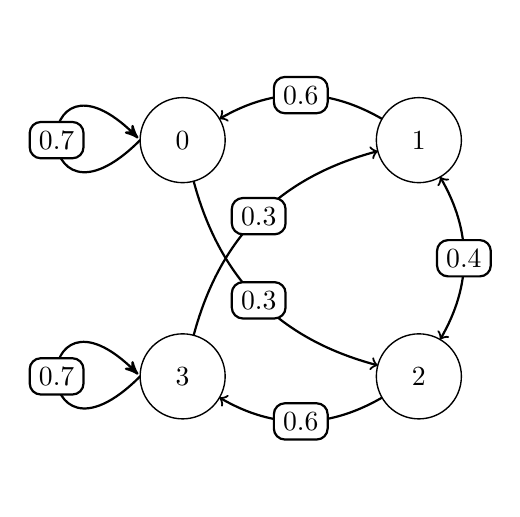
\begin{tikzpicture}
		%\node[draw,circle] at (1,1){$0$};
		\SetGraphUnit{3}
		\tikzset{LabelStyle/.style = {rectangle,rounded corners, draw, fill=white!50},
		VertexStyle/.append style={inner sep=8pt}}
		\Vertex{0}
		\EA(0){1}
		\SO(0){3}
		\SO(1){2}
		\tikzset{EdgeStyle/.append style = {->, bend right}}
		\Edge[label=0.6](1)(0)
		\Edge[label=0.3](0)(2)
		\tikzset{EdgeStyle/.append style = {->, bend left}}
		\Edge[label=0.3](3)(1)
		\Edge[label=0.6](2)(3)
		\tikzset{EdgeStyle/.append style = {<->,bend right}}
		\Edge[label=0.4](2)(1)
		\Loop[dist=2cm, dir=NO, label=0.7](0.west)
		\Loop[dist=2cm, dir=NO, label=0.7](3.west)
	\end{tikzpicture}
	\caption{Markov chain model}
	\end{figure}
	
	\subsection{Part B}
	Find the probability that the first future loss will be followed by another loss.\\
	\\
	Since we are starting in state 3, the first future loss will put us in state 1. The probability that another loss will follow is the probability of moving from state 1 to state 0, which is 0.6.
	\\
	\subsection{Part C}
	Let $X$ be the number of games played up to, but not including, the first loss. Find the PMF of $X$.\\
	\\
	This is the same as the number of games in the initial winning streak. Since we start in state 3, the minimum value of $X$ is 2, with a probability of 0.3 since losing the next game will result in 2 wins. For each game won beyond, we multiply by a probability of 0.7. Thus, the PMF is
	\[
	p_X(x) =
	\begin{cases}
		(0.3)(0.7)^{x-2} & x \geq 2\\
		0 & \text{otherwise}
	\end{cases}
	\]
	\subsection{Part D}
	Either evaluate the steady state probabilities, or explain why they do not exist.\\
	\\
	The calculation of $[\pi_0~\pi_1 ~\pi_2~\pi_3]$ evaluates to finding the eigenvector of $P^T$ corresponding to the eigenvalue of 1. $P$ is the probability matrix of the Markov Chain, where $p_{ij}$ is the probability of moving from state $i$ to $j$. The eigenvector must then be normalized by the sum of the elements.
	
	This results in $[\pi_0~\pi_1 ~\pi_2~\pi_3] = [\frac{1}{3}~\frac{1}{6}~\frac{1}{6}~\frac{1}{3}]$
	\\
	\subsection{Part E}
	Find a good approximation that the team will win it's $1000^{th}$ game, given that the outcomes of games 1000 and 1001 are the same.\\
	\\
	Assuming that 1000 games is enough to reach the steady state probabilities, the probability of both game 1000 and game 1001 being won is the same as the probability of being in state 3. The probability of both games being the same is the sum of the probabilities of being in state 3 or state 0. Thus, the probability is
	\[
	\frac{\pi_3}{\pi_0 + \pi_3} = \frac{1/3}{1/3~+~1/3} = \frac{1}{2}
	\]
	\subsection{Part F}
	Let $T$ be the number of games up to and including the team's 2nd consecutive loss. What is $\mathbf{E}[T]$?\\
	\\
	In this situation, we must modify the Markov Chain to make state 0 an absorbing state, as shown below.
	\begin{figure}[h!]
		\centering
		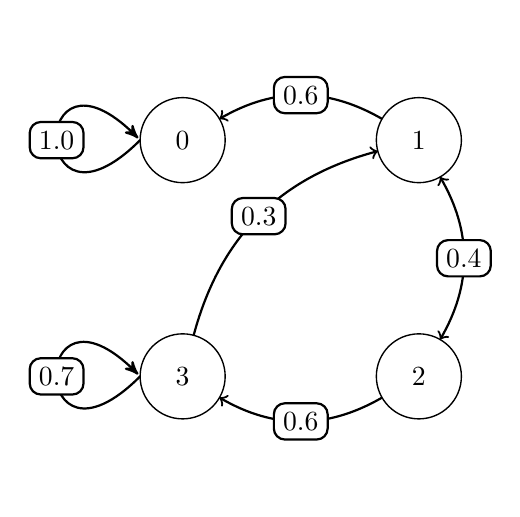
\begin{tikzpicture}
		%\node[draw,circle] at (1,1){$0$};
		\SetGraphUnit{3}
		\tikzset{LabelStyle/.style = {rectangle,rounded corners, draw, fill=white!50},
			VertexStyle/.append style={inner sep=8pt}}
		\Vertex{0}
		\EA(0){1}
		\SO(0){3}
		\SO(1){2}
		\tikzset{EdgeStyle/.append style = {->, bend right}}
		\Edge[label=0.6](1)(0)
		%\Edge[label=0.3](0)(2)
		\tikzset{EdgeStyle/.append style = {->, bend left}}
		\Edge[label=0.3](3)(1)
		\Edge[label=0.6](2)(3)
		\tikzset{EdgeStyle/.append style = {<->,bend right}}
		\Edge[label=0.4](2)(1)
		\Loop[dist=2cm, dir=NO, label=1.0](0.west)
		\Loop[dist=2cm, dir=NO, label=0.7](3.west)
		\end{tikzpicture}
		\caption{Markov chain model with state 0 as an absorbing state.}
	\end{figure}

	States 1-3 are transient states since they each reach state 0, but are not reachable by state 0. State 0 itself is a recurrent state. Thus the expected time to reach absorption starting at state 0, $\mu_0$ is 0.
	
	For the $i$th state of $m$ total states, the expected time to reach absorption is $\mu_i = 1+ \sum_{j=0}^{m}p_{ij}\mu_j$. Therefore we get the following system of equations:
	\[
		\begin{cases}
		\mu_0 = 0\\
		\mu_1 = 1 + 0.4\mu_2\\
		\mu_2 = 1 + 0.4\mu_1 + 0.6\mu_3\\
		\mu_3 = 1 + 0.3\mu_1 + 0.7\mu_3
		\end{cases}
	\]
	which can be represented in matrix form as
	\[
	\begin{bmatrix}
	1 & -0.4 & 0\\
	-0.4 & 1 & -0.6\\
	-0.3 & 0 & 0.3
	\end{bmatrix}
	\begin{bmatrix}
	\mu_1\\\mu_2\\\mu_3
	\end{bmatrix}
	=
	\begin{bmatrix}
	1\\1\\1
	\end{bmatrix}
	\]
	Since we start in state 3, $\mathbf{E}[T] = \mu_3$, which evaluates to 7 games.
	\\
	\subsection{Part G}
	The team is removed from competition after 3 losses in a row. Let $N$ be the number of games that the team will play in competition. What is $\mathbf{E}[N]$?\\
	\\
	We must add another state to the original Markov chain that signifies losing after being in state 0, shown below.
	\begin{figure}[h!]
		\centering
		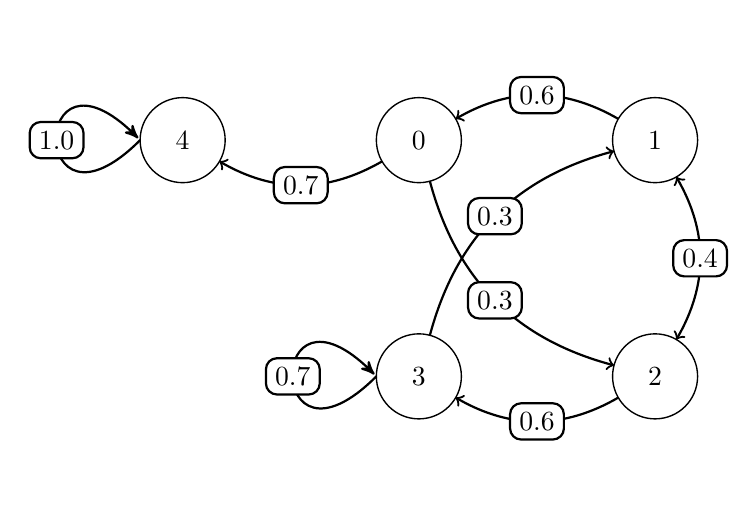
\begin{tikzpicture}
		%\node[draw,circle] at (1,1){$0$};
		\SetGraphUnit{3}
		\tikzset{LabelStyle/.style = {rectangle,rounded corners, draw, fill=white!50},
			VertexStyle/.append style={inner sep=8pt}}
		\Vertex{0}
		\EA(0){1}
		\SO(0){3}
		\SO(1){2}
		\WE(0){4}
		\tikzset{EdgeStyle/.append style = {->, bend right}}
		\Edge[label=0.6](1)(0)
		\Edge[label=0.3](0)(2)
		\tikzset{EdgeStyle/.append style = {->, bend left}}
		\Edge[label=0.3](3)(1)
		\Edge[label=0.6](2)(3)
		\Edge[label=0.7](0)(4)
		\tikzset{EdgeStyle/.append style = {<->,bend right}}
		\Edge[label=0.4](2)(1)
		\Loop[dist=2cm, dir=NO, label=1.0](4.west)
		\Loop[dist=2cm, dir=NO, label=0.7](3.west)
		\end{tikzpicture}
	\caption{Markov chain model with added absorbing state 4 for three losses in a row.}
	\end{figure}
	
	This new Markov chain results in the following systems of equations for average absorption times.
	\[
	\begin{cases}
	\mu_0 = 1 + 0.3\mu_2\\
	\mu_1 = 1 + 0.6\mu_0 + 0.4\mu_2\\
	\mu_2 = 1 + 0.4\mu_1 + 0.6\mu_3\\
	\mu_3 = 1 + 0.3\mu_1 + 0.7\mu_3\\
	\mu_4 = 0
	\end{cases}
	\]
	which is expressed as matrices by
	\[
	\begin{bmatrix}
	1    & 0    & -0.3 & 0\\
	-0.6 & 1    & -0.4 & 0\\
	0    & -0.4 & 1    & -0.6\\
	0    & -0.3 & 0    & 0.3\\
	\end{bmatrix}
	\begin{bmatrix}
	\mu_0\\\mu_1\\\mu_2\\\mu_3
	\end{bmatrix}
	=
	\begin{bmatrix}
	1\\1\\1\\1
	\end{bmatrix}
	\]
	which evaluates to $\mathbf{E}[N] = \mu_3 = 11.28$ games.
\end{document}